\documentclass[tikz,border=4pt]{standalone}
\usepackage{pgfplots}
\pgfplotsset{compat=1.18}
\definecolor{accB}{HTML}{1769AA}
\definecolor{fillB}{HTML}{DCEAF5}
\definecolor{accO}{HTML}{C85A00}
\definecolor{fillO}{HTML}{FCE8D5}
\definecolor{ink}{HTML}{18212B}
\definecolor{slate}{HTML}{66727D}
\definecolor{gridg}{HTML}{E4E7EA}
% note (luojiaxuan): memory-critical vs control 分组柱:一高一平的核心卖点图。
% 柱体浅色填充+主色描边(与图 1/2 的卡片语言一致),柱顶直标数值。
\begin{document}
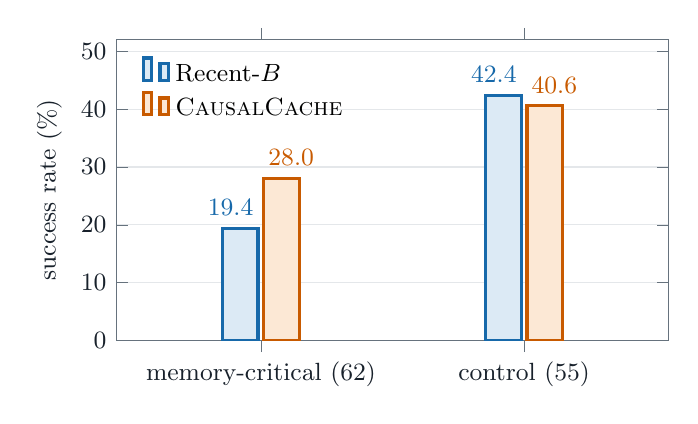
\begin{tikzpicture}
\begin{axis}[
  width=8.6cm, height=5.4cm,
  ybar, bar width=13pt,
  ylabel={success rate (\%)},
  ymin=0, ymax=52,
  xtick={0,1},
  xticklabels={memory-critical ($62$), control ($55$)},
  xmin=-0.55, xmax=1.55,
  ytick={0,10,20,30,40,50},
  axis line style={slate}, tick style={slate},
  ticklabel style={font=\small, color=ink},
  label style={font=\small, color=ink},
  ymajorgrids, grid style={gridg},
  legend style={at={(0.03,0.965)}, anchor=north west, font=\small,
    draw=none, fill=none},
  legend cell align=left,
]
\addplot[draw=accB, very thick, fill=fillB]
  coordinates {(0,19.4) (1,42.4)};
\addlegendentry{Recent-$B$}
\addplot[draw=accO, very thick, fill=fillO]
  coordinates {(0,28.0) (1,40.6)};
\addlegendentry{\textsc{CausalCache}}
% 柱顶数值
\node[font=\small, text=accB, anchor=south] at (axis cs:-0.115,19.9) {19.4};
\node[font=\small, text=accO, anchor=south] at (axis cs:0.115,28.5) {28.0};
\node[font=\small, text=accB, anchor=south] at (axis cs:0.885,42.9) {42.4};
\node[font=\small, text=accO, anchor=south] at (axis cs:1.115,41.1) {40.6};
\end{axis}
\end{tikzpicture}
\end{document}
